\subsection{Defining the Problem}
For this last problem, we were instructed to investigate whether reduced usage of certain modes of transportation are a cause of E-Bike sales growth. We then had to quantify these resulting impacts on certain factors.

\subsection{The Model}
We quantified individual health benefits using our optimal regression function from section 1, the tilted sigmoid. Specifically, we performed cumulative projections for two- and five- year windows. This yielded the following results for the total number of e-bikes sold up to and including the maximum year, summarized in the table:

\begin{center}
    \begin{tabular}{ |c|c|c|c|}
        \hline
        \textbf{Year}  & \textbf{E-bike sales volume (to nearest integer)}\\
        \hline
        2025 & 11725\\
        \hline
        2028 & 30829\\
        \hline
    \end{tabular}
\end{center}

Research has indicated that e-bike use is associated with improvements in physical health. For instance, it constitutes moderate to vigorous exercise, requiring a higher heart rate and oxygen intake than activities such as walking. This improves overall cardiovascular health leading to overall improved health and mood, in turn leading to a better quality of life.

From an economic perspective, an increase in the quantity of e-bikes produced and consumed at the market equilibrium (i.e., where supply equals demand), results in a net welfare gain for society. Assuming e-bike use creates a positive externality (that is, a positive impact on a third party/society at large), the market can be illustrated econometrically as follows:

\begin{center}
    \makebox[\textwidth]{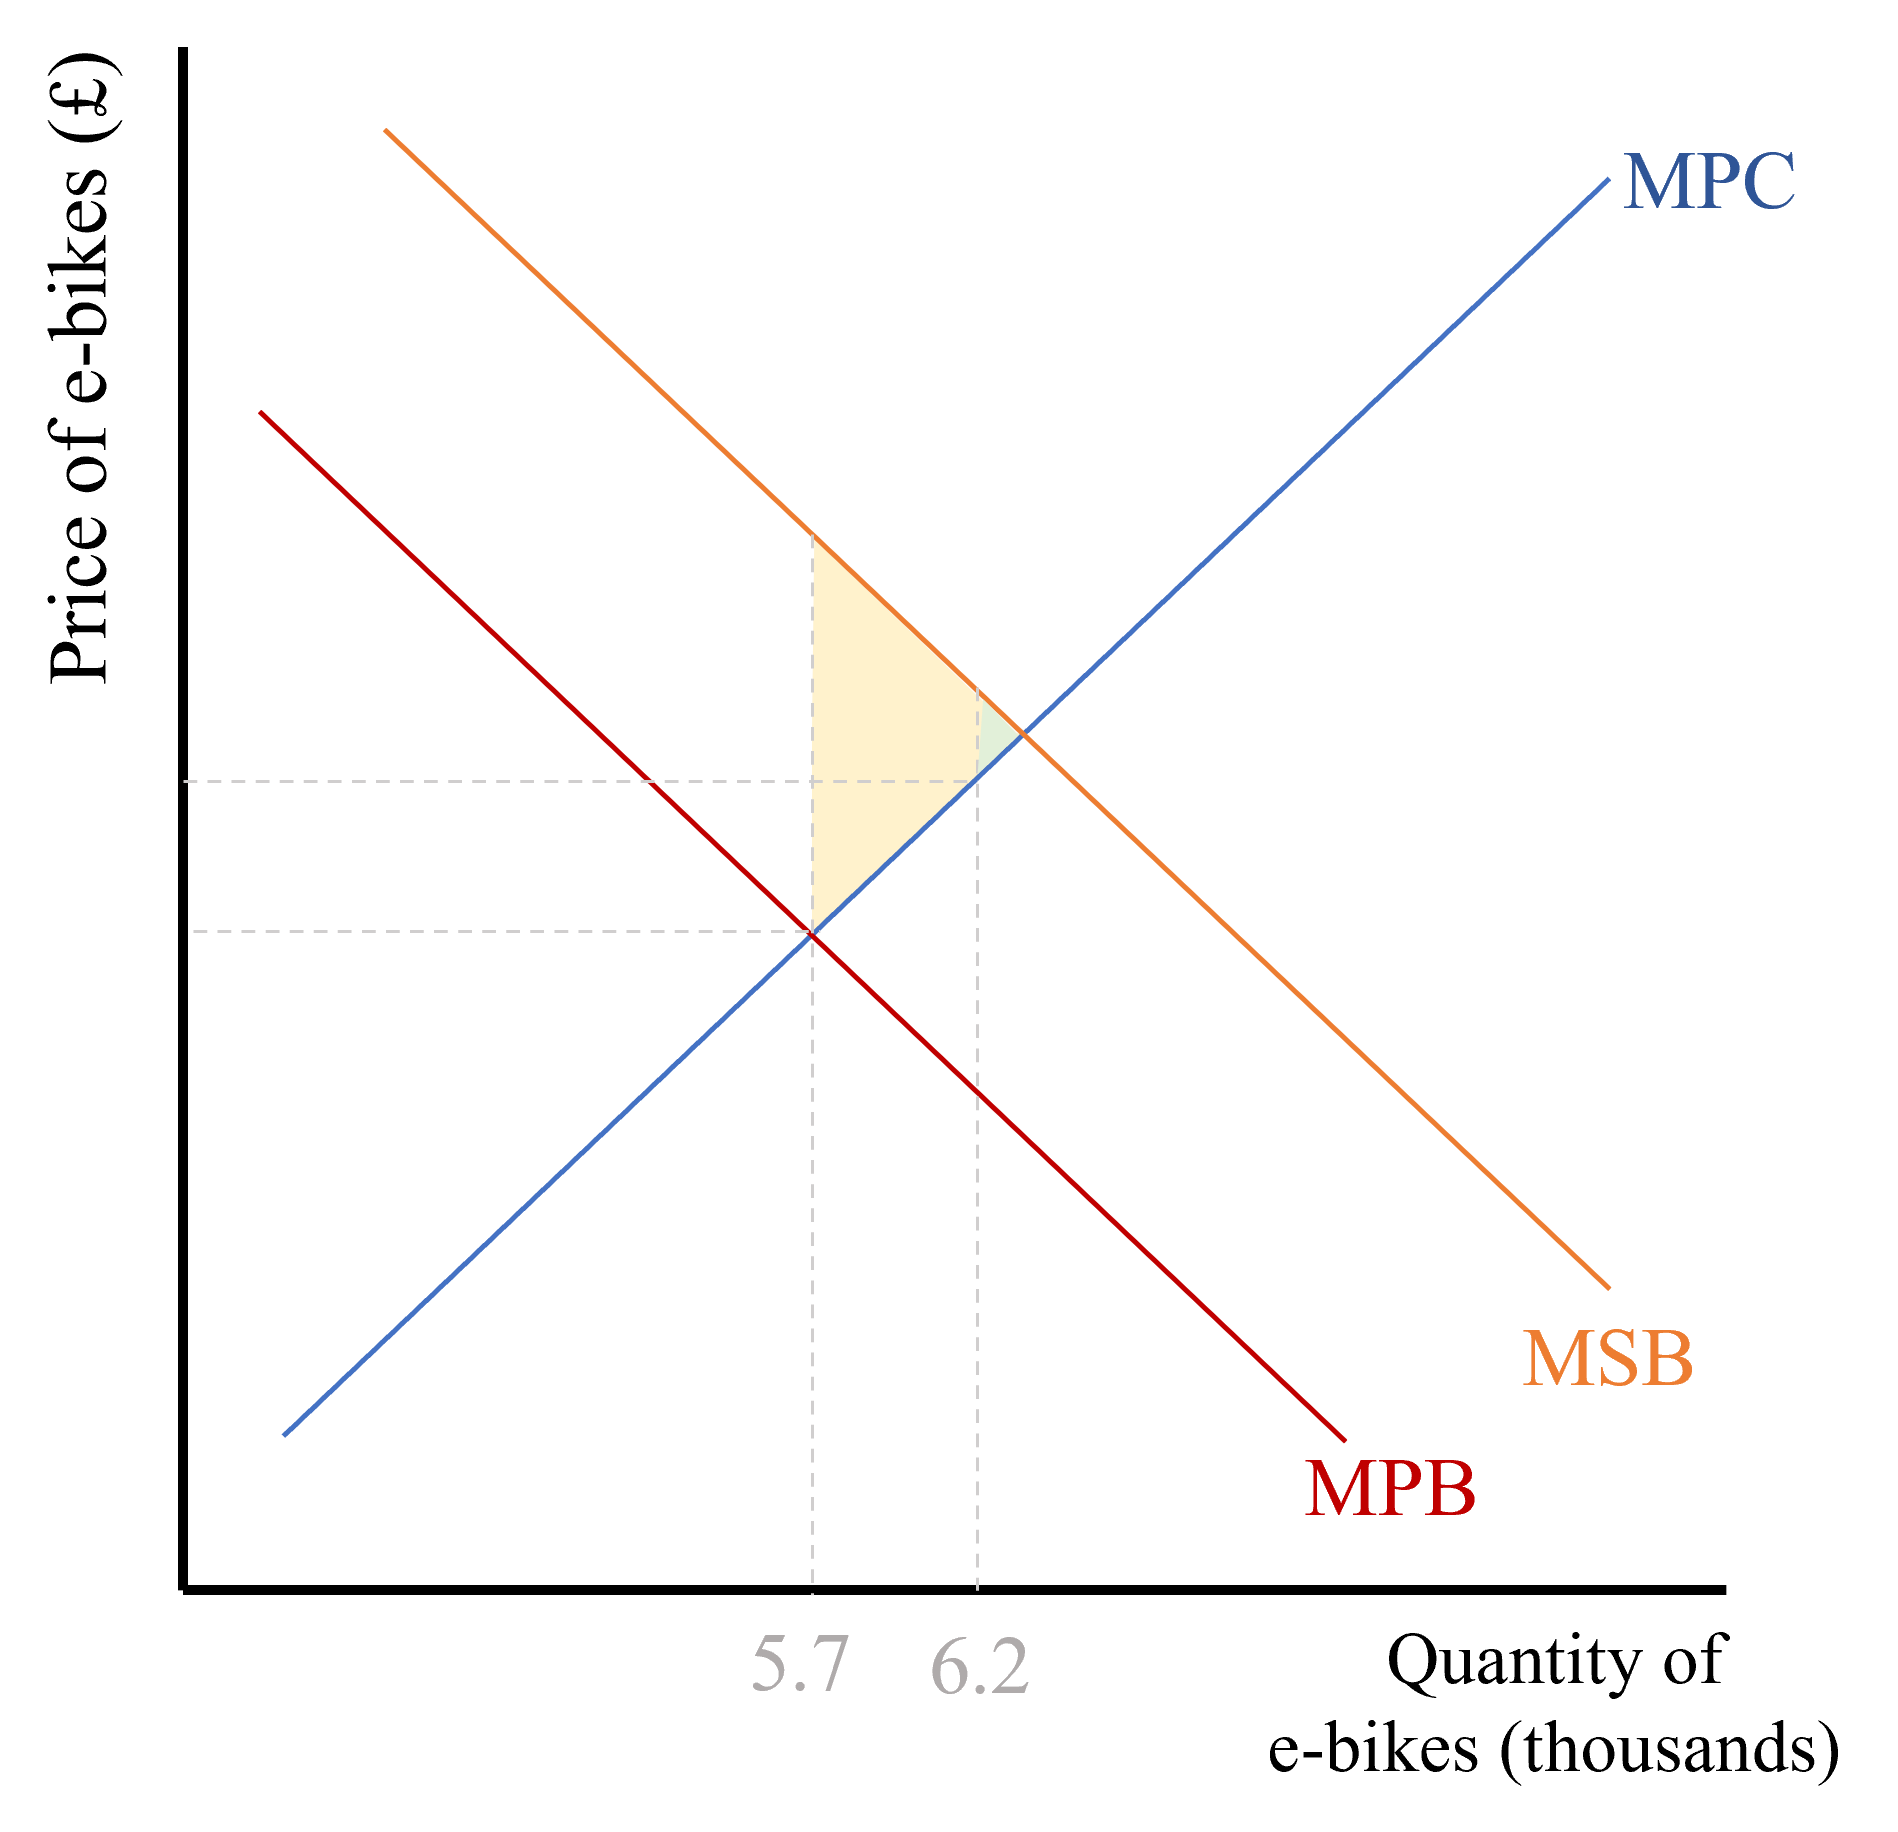
\includegraphics[width=\textwidth]{externality.png}}
\end{center}

The figure above depicts a simple economic visualisation of the market for e-bikes. The marginal private cost (proportional to supply) is shown in blue, the marginal private benefit (proportional to demand) is shown in red, and the marginal social benefit (proportional to demand + positive externalities) is shown in red. The initial welfare loss is shown by the yellow shaded trapezium + the green shaded triangle. Following the increase in quantity from approximately 5.7 to 6.2 thousand (from 2023-25), the welfare loss decreases and is indicated by the green shaded triangle. This indicates a welfare gain for society.

Amid the current economic climate and inflationary pressures, obtaining accurate figures for price changes for analysis proved to be difficult. For this reason, our analysis is semi-quantitative and based on fundamental economic theory; geometrically, it is easy to visualise the shrinking of the welfare loss as indicated by the shaded areas in the figure. 
Almost counterintuitively, we can conclude that individual health benefits in themselves result in societal gain. More practically, this could be due to reduced pressure on shared healthcare systems. 


\newpage
